\newcommand{\TeamNo}{31}

\newcommand{\HWno}{05}

\newcommand{\AuthorOneName}{Merve Nur Öztürk}
\newcommand{\AuthorOneID}{2311322}

\newcommand{\AuthorTwoName}{Atakan Süslü}
\newcommand{\AuthorTwoID}{2311371}

\newcommand{\AuthorThreeName}{Betül Rana Kuran}
\newcommand{\AuthorThreeID}{2311173}


\documentclass[letterpaper,12pt]{article}
\usepackage{tabularx} % extra features for tabular environment
\usepackage{amsmath}  % improve math presentation
\usepackage{amssymb}
\usepackage{xcolor}
\usepackage{float}
\usepackage[export]{adjustbox}
\usepackage{graphicx} % takes care of graphic including machinery
\usepackage[margin=1in,letterpaper]{geometry} % decreases margins
\usepackage{cite} % takes care of citations

\begin{document}
\begin{center}
AE 305, 2020-21 Fall \hfill \textbf{HW \HWno} \hfill \textbf{Team \TeamNo} \\
\noindent\rule{\textwidth}{0.4pt}
\begin{tabular}{p{0.33\textwidth} | p{0.33\textwidth} | p{0.33\textwidth} }
	\AuthorOneName&\AuthorTwoName&\AuthorThreeName\\
	\textit{\AuthorOneID}&\textit{\AuthorTwoID}&\textit{\AuthorThreeID}
\end{tabular}
\noindent\rule{\textwidth}{0.4pt}
\end{center}

%Report start

\section{Introduction}
Elliptic partial differential equations can be solved by using finite difference equations,
and the most common FDE for the solution of an elliptic PDE is obtained by second-order
central difference approximations of the derivatives. Afterwards, the FDE can
be solved either by direct solution methods or iterative methods. In this homework, a 2D
heat equation is given:

\begin{equation}
	\frac{\partial^2T}{\partial x^2} + \frac{\partial^2T}{\partial y^2} = 0
	\label{eqn:heateqn}
\end{equation}

It is requested to compute the steady state temperature distribution on a given 2D model
of a room having a width of 10m and a height of 6m by solving the above equation for 
two different cases, one is with a radiator and the other is without a radiator. First,
the iterative methods are used; Point Jacobi, Gauss-Seidel, SOR and Line Gauss-Seidel
methods, then the solution is obtained by the direct solution methods. For the final
solution, it is asked to plot the heat flux distribution in the room, and the heat flux
vector is given as follows:

\begin{equation}
	\vec{q} = -k \nabla T
	\label{eqn:heatflux}
\end{equation}

It is also asked to compare the convergence rates of the iterative methods.
\section{Method}
\section{Results and Discussion}

\subsection{Solution of the Heat Equation in the Absence of a Radiator}
\begin{figure}[H] 
	\centering 
	\includegraphics[max height=12cm]{graphs/point_norad/point_norad.png}
	\caption{Solution of the heat equation by Point Jacobi method.}
 	\label{fig:pointnorad}
\end{figure}
\begin{figure}[H] 
	\centering 
	\includegraphics[max height=12cm]{graphs/gauss_norad/gauss_norad.png}
	\caption{Solution of the heat equation by Gauss-Seidel method.}
 	\label{fig:gaussnorad}
\end{figure}
\begin{figure}[H] 
	\centering 
	\includegraphics[max height=12cm]{graphs/SOR_O19_norad/SOR_O19_norad.png}
	\caption{Solution of the heat equation by SOR method.}
 	\label{fig:sornorad}
\end{figure}
\subsubsection{Comparison of the Convergence Rates}
\begin{figure}[H] 
	\centering 
	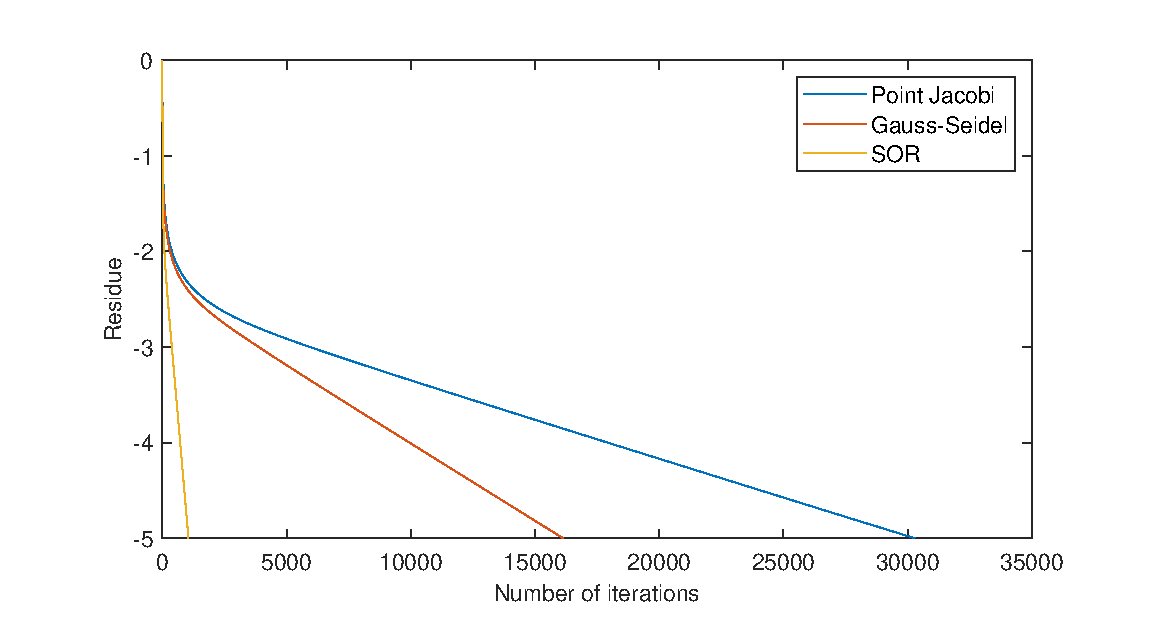
\includegraphics[max height=9cm]{graphs/residual_SOR19_norad.eps}
	\caption{Convergence rates of Point Jacobi, Gauss-Seidel and SOR methods.}
 	\label{fig:convnorad}
\end{figure}
\subsubsection{Temperature Distributions along x=5m and y=3m}
\begin{figure}[H] 
	\centering 
	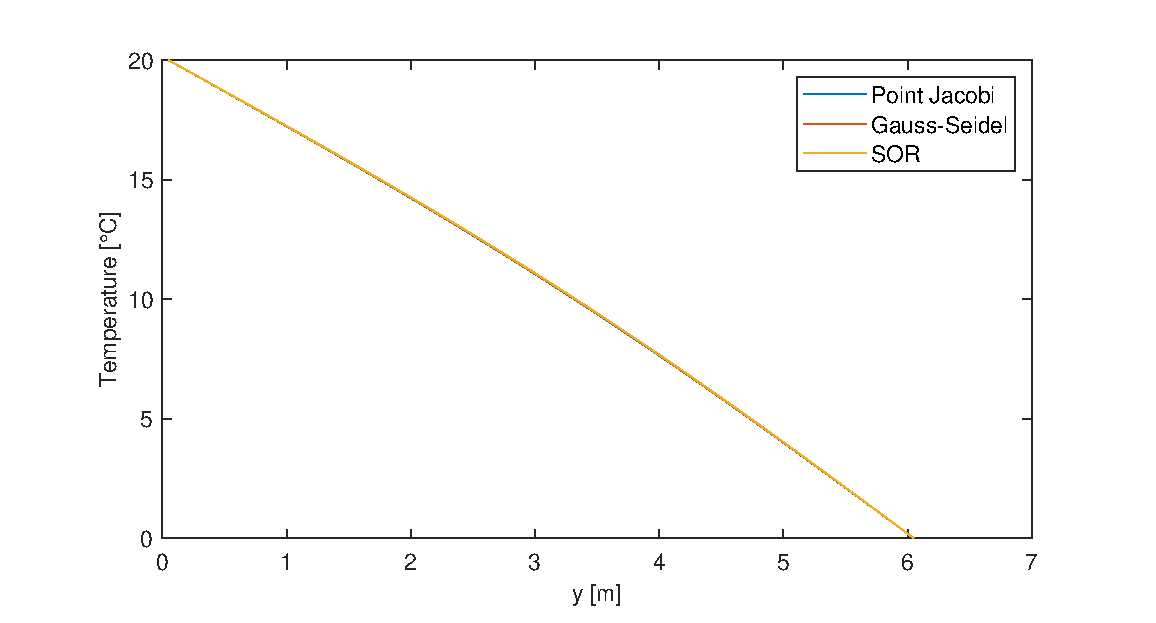
\includegraphics[max height=9cm]{graphs/x5_SOR19_norad.eps}
	\caption{Temperature distributions along x=5m}
 	\label{fig:x5norad}
\end{figure}
\begin{figure}[H] 
	\centering 
	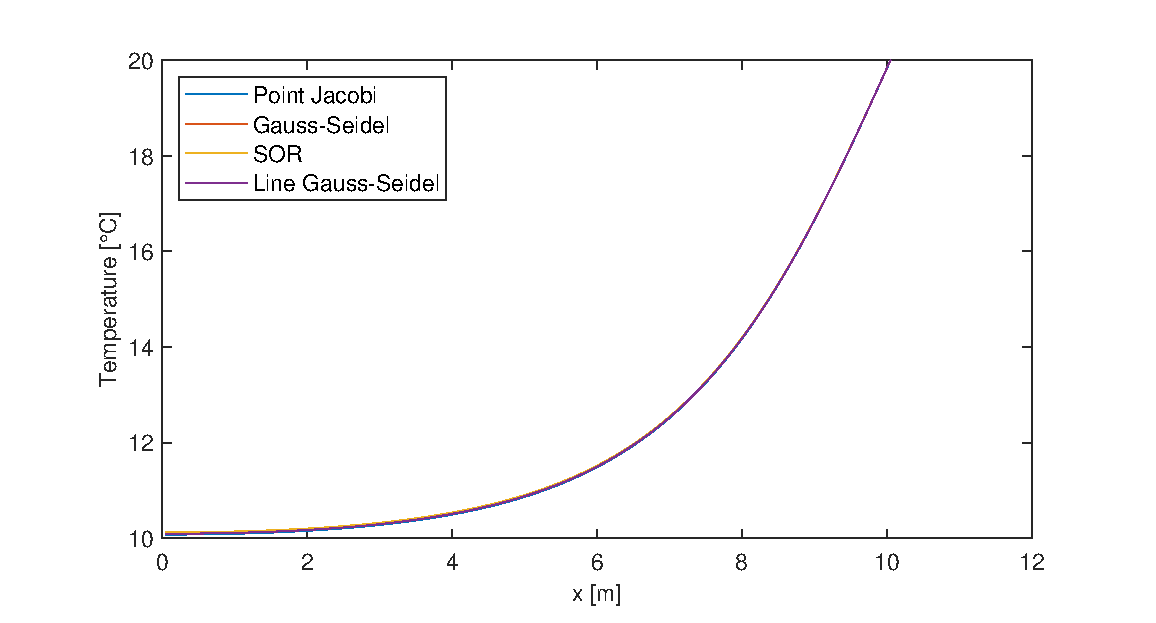
\includegraphics[max height=9cm]{graphs/y3_SOR19_norad.eps}
	\caption{Temperature distributions along y=3m}
 	\label{fig:y3norad}
\end{figure}

\subsection{Solution of the Heat Equation with Existence of a Radiator}
\begin{figure}[H] 
	\centering 
	\includegraphics[max height=12cm]{graphs/point_rad_default/point_rad_default.png}
	\caption{Solution of the heat equation by Point Jacobi method.}
 	\label{fig:pointrad}
\end{figure}
\begin{figure}[H] 
	\centering 
	\includegraphics[max height=12cm]{graphs/gauss_rad_default/gauss_rad_default.png}
	\caption{Solution of the heat equation by Gauss-Seidel method.}
 	\label{fig:gaussrad}
\end{figure}
\begin{figure}[H] 
	\centering 
	\includegraphics[max height=12cm]{graphs/SOR_O19_rad_default/SOR_O19_rad_default.png}
	\caption{Solution of the heat equation by SOR method.}
 	\label{fig:sorrad}
\end{figure}
\subsubsection{Comparison of the Convergence Rates}
\begin{figure}[H] 
	\centering 
	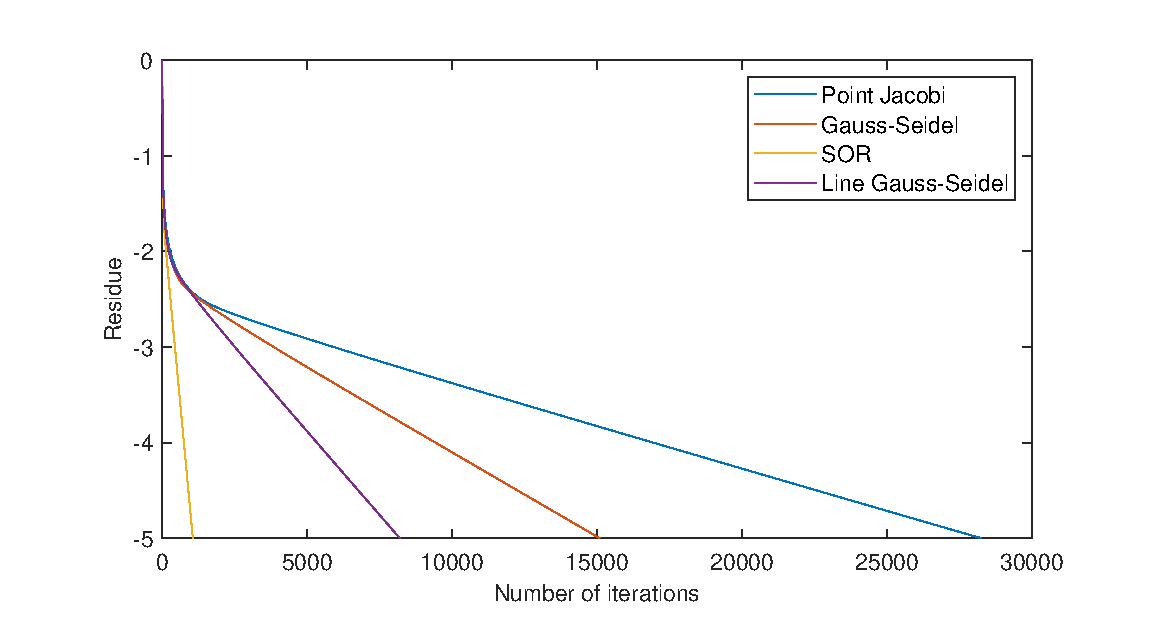
\includegraphics[max height=9cm]{graphs/residual_SOR19_defaultrad.eps}
	\caption{Convergence rates of Point Jacobi, Gauss-Seidel and SOR methods.}
 	\label{fig:convrad}
\end{figure}
\subsubsection{Temperature Distributions along x=5m and y=3m}
\begin{figure}[H] 
	\centering 
	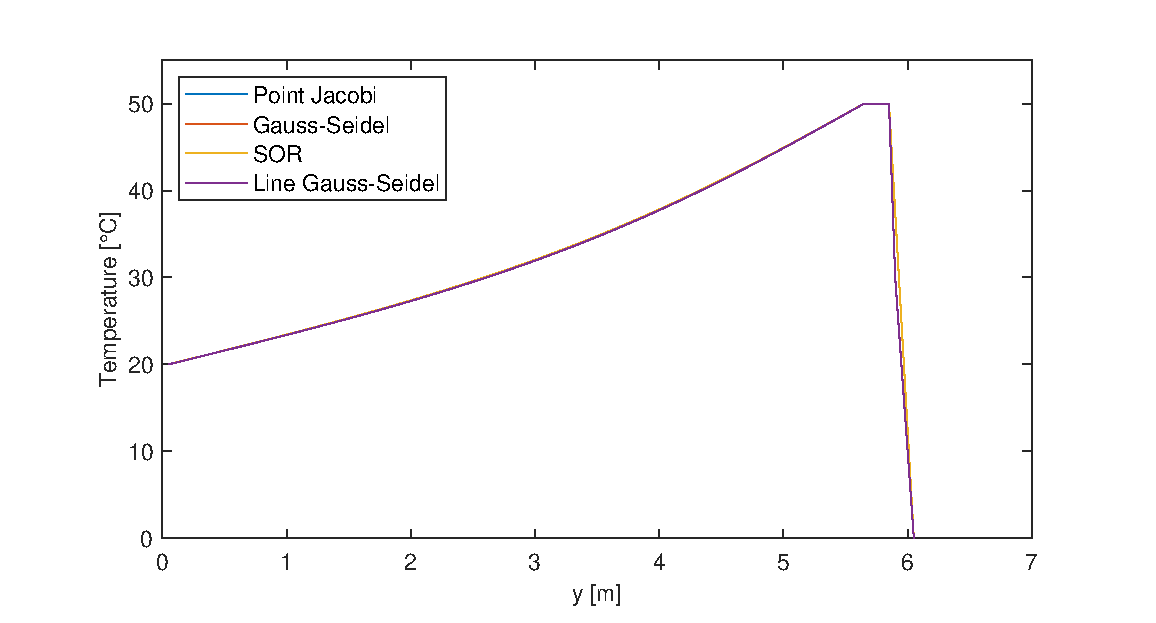
\includegraphics[max height=9cm]{graphs/x5_SOR19_defaultrad.eps}
	\caption{Temperature distributions along x=5m}
 	\label{fig:x5rad}
\end{figure}
\begin{figure}[H] 
	\centering 
	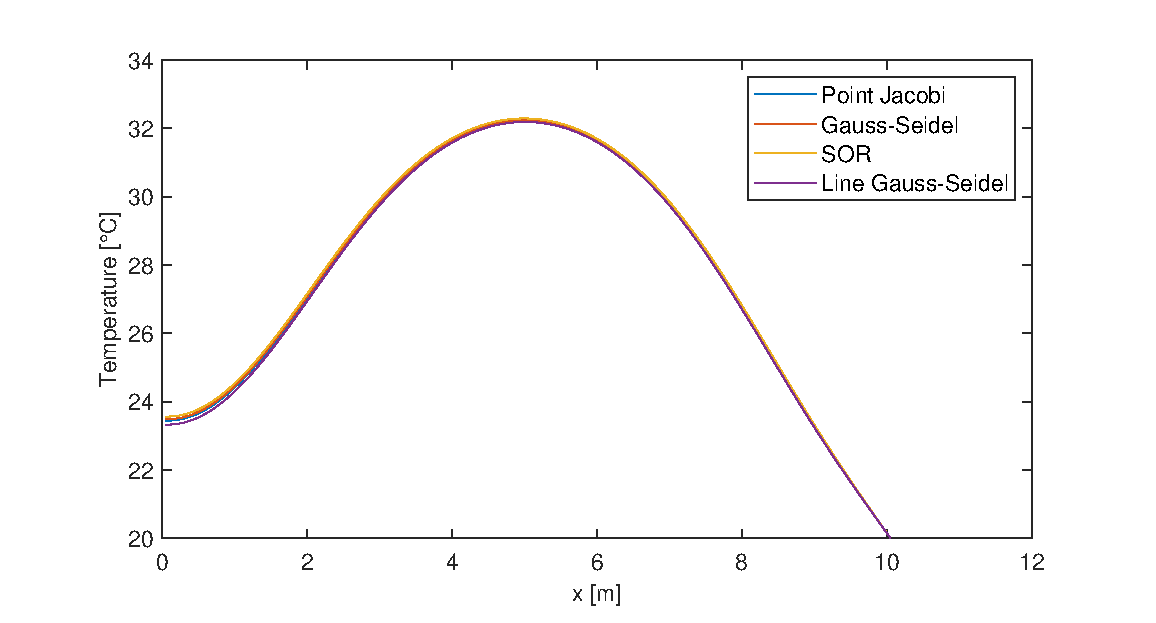
\includegraphics[max height=9cm]{graphs/y3_SOR19_defaultrad.eps}
	\caption{Temperature distributions along y=3m}
 	\label{fig:y3rad}
\end{figure}

\section{Conclusion}
\end{document}